\chapter{The consequences of a thermal shield}\label{cha:the-shield}

Why a shield, what does the shield do, maybe short introduction


- Small shield maybe better

- Difference between small and large shield
  
  -- Small shield: Take maximum (or minimum) and this is the casimir force. This is the same as just a angle $\Delta \theta$
  
  -- Large shield: $\Delta \theta$ and $\Delta L$

  -- Use linearity of arctan and central-limit-theorem: This angle is the same as always above

- Entanglement generated by the shield

- Entanglement dynamics with extra shield vibrations


\section{Thickness and size of the shield}\label{sec:5:shield-size}
The thickness $d$ and the radius $r_s$ of the spherical shield can be estimated by considering the properties of a physical conductive material with high electrical conductivity $\sigma$.
Even a superconducting shield could be considered for an almost perfect shielding of electromagnetic fields.
The transmission $T$ of electromagnetic waves through a physical shield is given by \cite{Vandenbosch_2022}
\begin{equation}
  T = \abs{\frac{\vec{E}_\mathrm{after}}{\vec{E}_\mathrm{before}}} = \frac{2}{Z_0 \sigma d}
\end{equation}
where $Z_0 = 377\si{\Omega}$ is the impedance of free space (assuming the shield is placed in a vacuum or in air).
The electric conductivity $\sigma$ is highly dependent on the temperature \cite[p. 284-286]{Gross_2018}, decreasing approximately with $1/T^5$ at low temperatures \footnote{This behavior is valid for temperatures below the Debye temperature ($\Theta_D = 343\si{K}$ for copper). At the low temperatures used in the experiment, this model accurately describes the conductivity of metals \cite{Berman_1952}.}.
Copper offers a strong electric conductivity of $\sigma = 59.6\times 10^6 \si{S/m}$ at room temperature and measured data showing even $\sigma(T = 10\si{K}) \approx 1.5\times 10^{10}\si{S/m}$ at $10\si{K}$ \cite{Berman_1952}.

To estimate the shield's thickness, the primary criterion used, is that gravitational interactions should dominate the entanglement generation.
Other mutual interactions between the particles, such as Coulomb or Casimir forces, must be sufficiently suppressed by the shield.
The \emph{entanglement rate} $\Gamma$ quantifies the build-up of entanglement over time
\begin{equation}\label{eq:5:entanglement-rate}
  \Gamma = \dv{t} E_N(\rho)\Big|_{t=0} \, ,
\end{equation} 
where $E_N$ is an appropriate entanglement measure - in this case the logarithmic negativity \cite{Plenio_2005} introduced in \cref{sec:2:entanglement-measures}.
For gravitational interactions, the entanglement rate in the parallel orientation is given by using eq. \eqref{eq:2:entanglement-dynamics-parallel} as
\begin{equation}\label{eq:5:entanglement-rate-gravity}
  \Gamma_\mathrm{Gravity} = \frac{G M_A M_B \Delta x_A \Delta x_B}{16 \hbar L^3 \log 2} = \frac{G \pi^2 R^6 \rho_\mathrm{Silica}^2 (\Delta x)^2}{9 \hbar L^3 \log 2} .
\end{equation}
where in the last step $M_A = M_B = 4/3 \pi R^3 \rho_\mathrm{Silica}$ and $\Delta x_A = \Delta x_B \equiv \Delta x$ was used.
The entanglement rate for non-gravitational interactions, such as Coulomb or Casimir forces, must be significantly smaller than the gravitational entanglement rate, ideally by a factor $\chi > 1$.
This ensures that the measured entanglement is primarily due to gravitational interactions.
In the following sections, estimations about the thickness and size of the shield are made, to effectively screen Coulomb and Casimir forces.


\subsection{Shielding Coulomb-Interactions}
The primary role of the Faraday shield is to block electromagnetic interactions between particles.
Experimentally, it may be beneficial for the particles to carry a small amount of charge, enabling the use of electrostatic traps with high trapping strength and large controllability \cite{GonzalezBallestero_2021}. 
The Coulomb interaction potential between two charged particles is given by
\begin{equation}
  V = \frac{1}{4\pi\varepsilon_0} \frac{q_A q_B}{2L}
\end{equation}
where $\varepsilon_0 = 8.8542\times 10^{-12}\si{A^2 s^4 m^{-3} kg^{-1}}$ is the permittivity of free space and $\abs{q_{A(B)}} = e = 1.6022\times 10^{-19}\si{C}$ the charge of particle $A$ and $B$ respectively.
This interaction mimics the form of the gravitational potential and can similarly induce entanglement with a entanglement rate
\begin{equation}\label{eq:5:entanglement-rate-coulomb}
  \Gamma_\mathrm{Coulomb} = \frac{T \abs{q_A q_B} (\Delta x)^2}{64 \pi \varepsilon_0 \hbar L^3 \log 2} .
\end{equation}
The shield suppresses the coupling by a factor of $T$.
Requiring $\Gamma_\mathrm{Gravity} > \chi \Gamma_\mathrm{Coulomb}$, the minimum thickness of the shield can be calculated as
\begin{align}\label{eq:5:coulomb-gravity-condition}
  T \frac{\abs{q_A q_B}}{64 \pi \varepsilon_0} \chi \, &< \, \frac{G \pi^2 R^6 \rho_\mathrm{Silica}^2}{9} \\
  \Longleftrightarrow \quad\quad\quad\quad d \, &> \, \frac{9}{32}\frac{1}{Z_0 \sigma} \frac{1}{\pi^3 \varepsilon_0 G \rho_\mathrm{Silica}^2} \frac{e^2}{R^6} \chi .
\end{align}
The thickness strongly depends on the particles size $R$, and large or heavy particles will favor gravitational entanglement generation.
Assuming the particles are silica nano-spheres with parameters given in \cref{tab:paramters}, a minimum shield-thickness of $d \approx 10\si{nm}\chi$ at $4\si{K}$ and of $d \approx 2.5\si{\mu m}\chi$ at room temperature is required.
At low temperatures, a realistic shield thickness could therefore be $d=100\si{nm}$, balancing engineering practicality and electromagnetic suppression.
Exact estimations however depend on the realization of the experiment as well as the precision in which the evolved state is measurable.

Electrostatic fields still can propagate around the finite-sized Faraday shield and potentially induce entanglement.
It is possible to estimate the required shield radius $r_s$ to block a specific amount $\eta$ of the electric field (see \cref{apx:blocking-of-the-shield}):
\begin{equation}\label{eq:5:shield-effectiveness}
  \frac{r_s}{L} = \sqrt{\frac{1-(1-\eta)^2}{(1-\eta)^2}}
\end{equation}
The results are visualized in \cref{fig:5:shield-radius}.
\begin{figure}[!ht]
  \centering
  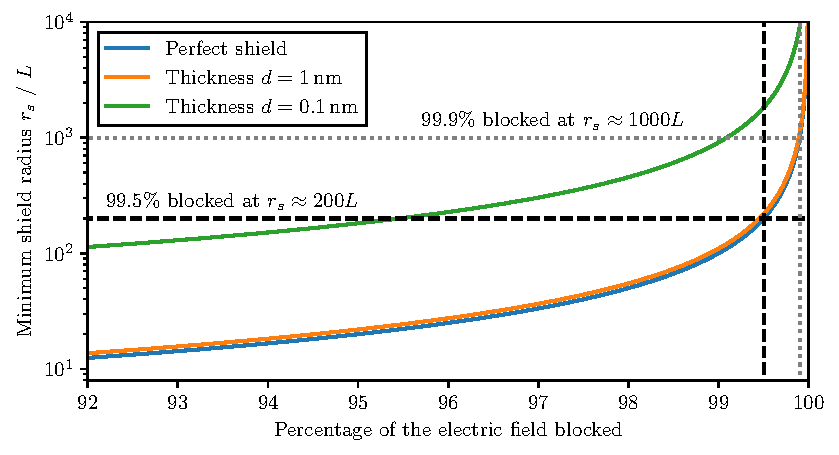
\includegraphics[width=\textwidth]{./../figures/others/shield-radius.pdf}
  \caption{Shield radius as a function of the shielding effectiveness $\eta$ for an ideal shield. Additionally, a real shield with varying thicknesses $d$ is considered at $T=300\si{K}$.
  To achieve shielding of $99.5-99.9\%$ ($\eta = 0.995-0.999$), a radius of $r_s =200-1000L$ is needed.}
  \label{fig:5:shield-radius}
\end{figure}
The shield's transmission $T$ should therefore be modified to $\tilde{T} = T\eta + (1-\eta)$, where the shielding effectiveness $\eta$ depends on $r_s$ as given by eq. \eqref{eq:5:shield-effectiveness}.
Modifying eq. \eqref{eq:5:coulomb-gravity-condition}, a minimum effectiveness $\eta_\mathrm{min}$ for sufficient shielding of
\begin{equation}
  \eta_\mathrm{min} \approx 1 - \frac{64\pi^3 \varepsilon_0 G R^6 \rho^2_\mathrm{Silica}}{9 e^2}
\end{equation}
can be approximated.
Using again the parameters from \cref{tab:paramters}, a minimum shielding of $\eta_\mathrm{min} \gtrsim 0.99997$ and thus a radius of $r_s \gtrsim 28000 L \approx 60\si{cm}$ is required.
Such a shield is too large for all practical purposes and it might be beneficial to choose heavier masses ($\tilde{M} \sim 4 M$) to reduce the shield size to the orders of $\sim 1\si{cm}$.
Due to practicality, a shield with $r_s = 1\si{cm}$ is used in the following calculations.
Uncharged particles would eliminate the Coulomb interactions and therefore reducing the shield's size and thickness to only shield mutual Casimir interactions.




\subsection{Shielding Casimir-Interactions}
Similarly to Coulomb interactions, it is possible to to estimate the required thickness for a shield to sufficiently block Casimir interactions.
The Casimir potential between the spheres with radius $R$ separated by $2L$ is given by \cite{Emig_2007}
\begin{equation}
  V = -\frac{23 \hbar c}{4\pi \cdot 128 L^7} \left( \frac{\varepsilon_r - 1}{\varepsilon_r + 2} \right)^2 R^6 .
\end{equation}
The corresponding entanglement rate is calculated similar to before by expanding the potential in small $\Delta x$ and computing the logarithmic negativity:
\begin{equation}
  \Gamma_\mathrm{Casimir} = T^2 \frac{161}{4096} \frac{c R^6 (\Delta x)^2}{\pi L^9 \log 2}\left( \frac{\varepsilon_r - 1}{\varepsilon_r + 2}\right)^2 .
\end{equation}
The dependence on $T^2$ arises because Casimir forces are second order effects in the dipole-dipole interaction \cite{Bordag_2001}.
Requiring gravitational entanglement generation to dominate, $\Gamma_\mathrm{Gravity} > \chi \Gamma_\mathrm{Casimir}$, leads to
\begin{align}
  T^2 \frac{161 c R^6}{4096 \pi L^6} \left( \frac{\varepsilon_r - 1}{\varepsilon_r + 2}\right)^2 \chi \, &< \, \frac{G \pi^2 \rho_\mathrm{Silica}^2 R^6}{9\hbar} \\
  \Longleftrightarrow \quad\quad\quad\  d \, &> \, \sqrt{\frac{1449}{4096} \frac{c \hbar}{G \pi^3}} \frac{2}{Z_0 \sigma \rho L^3} \frac{\varepsilon_r - 1}{\varepsilon_r + 2} \sqrt{\chi} .
\end{align}
For large separations, the shield thickness can be arbitrarily low, as Casimir forces vanish and at separations of $L\gtrsim 100\si{\mu m}$, the shield might not be required at all (compare \cref{sec:2:experimental-problems}).
Assuming two identical silica nano-spheres with parameters given by \cref{tab:paramters}, the required minimum thickness is between $4\times 10^{-11}\si{m} \sqrt{\chi}$ at $4\si{K}$ and $10 \si{nm} \sqrt{\chi}$ at room temperature.
This is much thinner than what is required for shielding Coulomb interactions.
The factor $\varepsilon_r$ modifies the thickness only by up to a constant factor of $\leq 1$ and is therefore ignored for worst-case estimations.

However, very thin shields lose mechanical rigidity, leading to enhanced vibrational excitations and potential instabilities.
Vibrational frequency and thus the vibrational energy depends linearly on the shield's thickness, making thinner shields prone to large decoherence due to thermal vibrations.
A detailed analysis of these effects is provided in the subsequent section.



\subsection{Gravitational effects of the shield}\label{subsec:5:shield-gravitation}
The gravitational interaction between the masses and the shield is generally neglected because it has no significant impact on the entanglement generation between the particles.
The only potential effect is indirect entanglement mediated by the thermal oscillations of the shield, as both masses couple gravitationally to it. 
However, as shown in \cref{sec:5:thermal-entanglement}, this second-order effect is very weak and does not pose a problem, since it still represents gravitationally mediated entanglement - which is the focus of the experiment anyway.
The gravitational force between a sphere with mass $M$ and a infinitesimal mass segment $\dd m = r d \rho_\mathrm{Cu} \dd r \dd \varphi$ of the shield made of copper with density $\rho_\mathrm{Cu} = 8960\si{kg/m^3}$ at a distance $r$ from the shield's center is given by
\begin{equation}
  \dd \vec{F} = \frac{G M \dd m}{\ell} \boldsymbol{\hat{\ell}} 
  \quad \Rightarrow \quad
  \dd F_z = \frac{G M r \rho_\mathrm{Cu} d}{\ell^2} \dd r \dd \varphi \cos \theta,
\end{equation}
where $\ell^2 = r^2 + L^2$ denotes the distance between the sphere and the mass segment and $\theta = \arccos L/\ell$ is the angle between them.
The total attractive force between the mass and the shield with radius $r_s$ is therefore
\begin{equation}
  F_z = GM \rho_\mathrm{Cu} d L \int\limits_{0}^{r_s} \dd r \int\limits_{0}^{2\pi} \dd \varphi \, \frac{r}{(r^2 + L^2)^{3/2}} = 2\pi G M \rho_\mathrm{Cu} d \left(1 - \frac{L}{\sqrt{L^2 + r_s^2}}\right) .
\end{equation}
For large shields $r_s \gg L$ this is independent of the particle-shield separation $L$.
For a shield with thickness $d = 100\si{nm}$ and the usual silica particle from \cref{tab:paramters}, the attraction force is around $F_\mathrm{particle-shield} \approx 4.1\times 10^{-24} \si{N}$ which is comparable with the attraction gravitational attraction force between the two particles themselves at $F_\mathrm{particle-particle} \approx 5.0 \times 10^{-24}\si{N}$ but is much weaker than the Casimir attraction between the particle and the shield with $F_\mathrm{Casimir} \approx 1.4 \times 10^{-17} \si{N}$.
Therefore, the gravitational effect of the shield can be neglected in all practical calculations.

\section{Thermal shield vibrations}\label{sec:5:thermal-vibrations}
A spherical plate with radius $r_s$ that is fixed at the edge can vibrate in different vibrational modes labeled by the indices $(k,l)$ where $k \in [1,\infty)$ and $l \in [0, \infty)$.
The exact vibrational frequency and the mode shape can only be given in terms of the Bessel functions. In fact, one of the first occurrences of these functions can be traced back to Euler trying to solve the very similar problem of a vibrating perfectly flexible membrane \cite{Dutka_1995}.
In general, the vibrations of a plate made out of a real material with thickness $d$ can be described by the differential equation \cite[p. 490]{Rao_2019}
\begin{equation}
  D \nabla^2\nabla^2 u = -\rho d \ddot{u}
\end{equation} 
where $D$ is given by material properties like Youngs module $E$ and the poisson number $\nu$ as
\begin{equation}
  D = \frac{d^3 E}{12(1-\nu^2)} .
\end{equation}
The general solution of this differential equation can be written in terms of the Bessel functions as (derived in Ref. \cite[p. 490-495]{Rao_2019}) 
\begin{equation}
  u_{kl}(r, \theta, t) = \left[J_l(\beta_k r) - \frac{J_l(\beta_k r_s)}{I_l(\beta_k r_s)}I_l(\beta_k r)\right]\cos(l\theta+\phi_1)\sin(\omega_{kl}t+\phi_2)
\end{equation}
with
\begin{equation} \label{eq:5:vibration-frequency}
  \beta_k = \frac{\tilde{r}_k}{r_s} \quad \text{and} \quad \omega_{kl} = \frac{\tilde{r}_k^2}{r_s^2}\sqrt{\frac{D}{\rho d}} = \tilde{r}_k^2\frac{d}{r_s^2}\sqrt{\frac{E}{12\rho(1-\nu^2)}} ,
\end{equation}
where $\tilde{r}_k$ is the $k$-th solution of the equation
\begin{equation}\label{eq:5:bessel-zeros}
  J_l(\tilde{r}_k)I_{l+1}(\tilde{r}_k)+I_l(\tilde{r}_k)J_{l+1}(\tilde{r}_k) = 0 .
\end{equation}
The phases $\phi_1$ and $\phi_2$ can be determined by initial conditions and refer to the rotation of the plate as well as temporal offsets. The shape of the first few modes is shown in \cref{fig:5:vibrational-modes}.
\begin{figure}[!htbp]
  \centering
  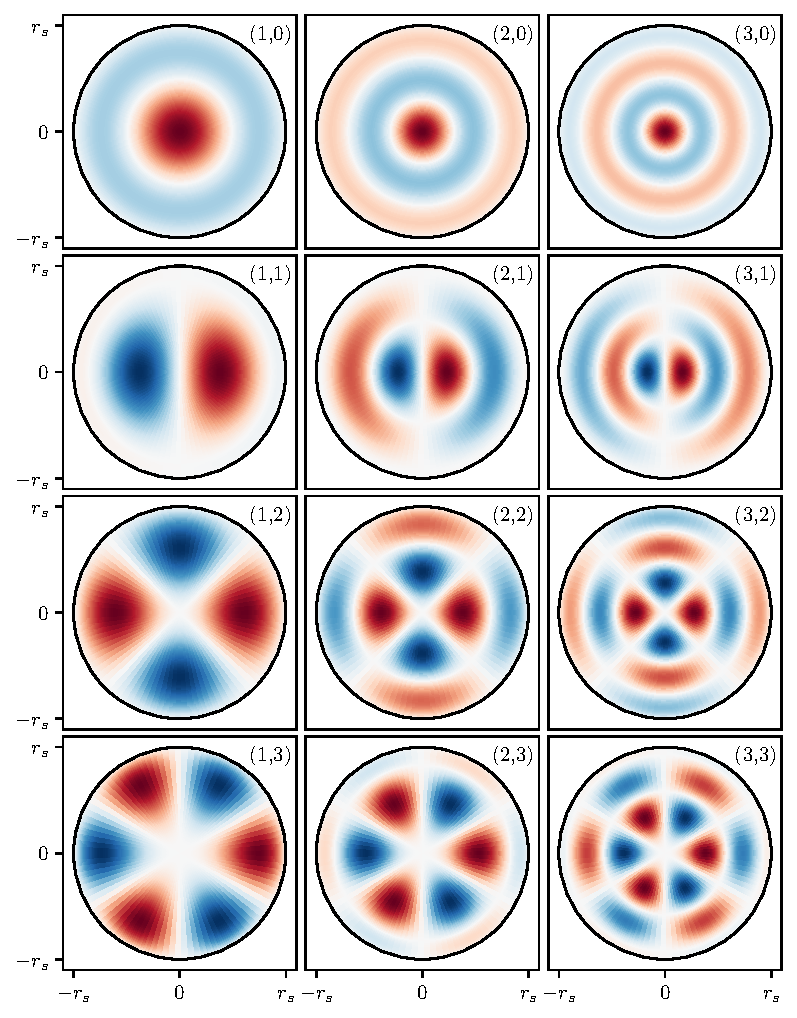
\includegraphics[width=\textwidth]{./../figures/vibrations/vibrational-modes-rd_bu.pdf}
  \caption{Shape of the first 12 modes $(k,l)$ ($k \geq 1$ and $l \geq 0$) of a vibrating spherical plate fixed at the edge with $r_s/d = 1000$.}
  \label{fig:5:vibrational-modes}
\end{figure}
In general, every possible vibration of the plates can be expressed as a sum of these default modes $u_{kl}$.
The amplitude $z$ of the vibrations are determined by the temperature $T$ and can be calculated by treating the amplitude of each vibration as a separate quantum harmonic oscillator with frequency $\omega_{kl}$.
The expectation value of the amplitude $\avg{z}$ is obviously zero and the variance $(\Delta z)^2 = \avg{z^2} - \avg{z}^2$ at temperature $T$ is given by (derivation in \cref{apx:thermal-harmonic-oscillator})
\begin{equation}\label{eq:5:amplitude-variance}
  (\Delta \op{z}_{kl})^2_T = \frac{\hbar}{2\tilde{m}\omega_{kl}}\coth(\frac{\hbar \omega_{kl}}{2k_BT}) \approx \frac{k_B T}{\tilde{m}\omega_{kl}^2} .
\end{equation}
In the last step $\hbar\omega \ll k_B T$ was used. $\tilde{m}$ is the \textit{effective mass} of the mode in which the precise shape is considered. A intuitive estimation for this mass can be given by the average amplitude of the mode 
\begin{equation}\label{eq:5:effective-mass}
  \tilde{m} = m\frac{1}{\pi r_s^2}\int\limits_0^{r_s} \dd r \int\limits_0^{2\pi} r\dd\theta \, u_{kl}(r, \theta, t)
\end{equation}
with $m=\rho \pi r_s^2 d$ being the total mass of the shield.
The amplitude of the plate vibrations are therefore in the order of $\Delta z_{kl} \propto \omega^{-1}$ at high temperatures or for low frequencies.




\subsection*{The effect of individual modes}
For a shield with radius $r_s = 1\si{cm}$ (in the following referred to as the \q{large shield}) and thickness $d=100\si{nmm}$ made out of Copper with $E = 110\si{GPa}$ and $\nu = 1/3$, the frequencies for the first few modes are between $11.0\si{s^{-1}}$ for $(1,0)$ up to $1018\si{s^{-1}}$ for like $(7,6)$.
These frequencies and thus the energy of the vibration $\hbar \omega$ is very small compared to the thermal energy $k_B T$ at all reasonable temperatures.
This means, that one expects a lot of modes to be substantially populated. Even at temperatures of $10^{-6} \si{K}$, the first $600$ modes are all equally likely to occur with a probability of $\approx 1/Z$ where $Z$ is the partition function
\begin{equation}
  Z = \sum_{m\in\{(k,l)\}} e^{-\beta \hbar \omega_m} .
\end{equation}

It is possible to calculate the asymptotic increase in the frequencies $\omega_{kl}$ for high modes $k \rightarrow \infty$.
This is, because the behavior for large inputs of the Bessel functions \cite[eq. 10.17.3]{DLMF}
\begin{equation}
  J_l(x) \sim \cos(x - \frac{l \pi}{2} - \frac{\pi}{4}) \quad \text{for} \ x \rightarrow \infty
\end{equation}
and modified Bessel functions \cite[eq. 10.40.1]{DLMF}
\begin{equation}
  I_l(x) \sim \frac{e^x}{\sqrt{2\pi x}} \quad \text{for} \ x \rightarrow \infty
\end{equation}
is known resulting in an asymptotic expansion of eq. \eqref{eq:5:bessel-zeros} 
\begin{equation}
  \sim \frac{e^x}{\sqrt{2\pi x}} \left[\cos(x - \frac{l \pi}{2} - \frac{\pi}{4}) + \cos(x - \frac{l \pi}{2} - \frac{3 \pi}{4})\right] = 0 .
\end{equation}
Therefore, the distribution of zeros $\tilde{r}_k$ is periodic for large $k$ as well as for large $l$.
The frequencies increase therefore with $\mathcal{O}(k^2 + l^2)$ for large modes.
The amplitude $\Delta z_\mathrm{kl} \propto 1/\omega$ therefore decreases quadratically with increasing mode order.
Therefore, even if at reasonable temperatures a lot of modes are occupied, the amplitude and thus the effect of each mode decreases for higher modes.
Additionally, because of the consideration of a real vibrating plate, the amplitude of the maximum of the shape $u_{kl}$ decreases for higher modes because the increased number of bulges require more material of the shield limiting the overall amplitude of the vibration even more.
Due to all these effects combined, it is sufficient to only consider the first few modes in all subsequent in numerical calculations.
However the effects of infinity many modes can be estimated asymptotically using the known scaling of $\omega_{kl}$ with increasing modes $(k,l)$.

It is also interesting to consider the scaling of the amplitudes $\Delta z$ for differently sized shields. 
According to eq. \eqref{eq:5:vibration-frequency}, the frequency $\omega$ increases quadratically with decreasing shield radius $r_s$.
However, the effective mass $\tilde{m}$ eq. \eqref{eq:5:effective-mass} depends also quadratically on the size of the shield resulting in a total dependence of $\Delta z \sim r_s$ for large temperatures and/or low modes.



% \subsection{OLDDD}


% \begin{equation}
%   \op{H} = \hbar \omega \left(\op{a}^\dagger\op{a} + \frac{1}{2}\right) + \tilde{g}_A(\op{z}) \ketbra{\psi_A} + \tilde{g}_B(\op{z}) \ketbra{\psi_B}
% \end{equation}

% Solution:
% \begin{equation}
%   \rho(t) = \frac{1}{2}\begin{pmatrix}
%     1 & e^{-i\varphi(t)}e^{-\gamma(t)}\\
%     e^{i\varphi(t)}e^{-\gamma(t)} & 1
%   \end{pmatrix}
% \end{equation}
% with the phase
% \begin{equation}
%   \varphi(t) = \frac{1}{\hbar^2\omega^2} \left(\sin(\omega t) - \omega t\right) \left(g_A^2 - g_B^2\right)
% \end{equation}
% and the decoherence term
% \begin{equation}
%   \gamma(t) = \frac{4(g_A - g_B)^2}{\hbar^2 \omega^2} \sin^2\left(\frac{\omega t}{2}\right) \left[\bar{n} + \frac{1}{2}\right]
% \end{equation}

% \begin{figure}[!htbp]
%   \centering
%   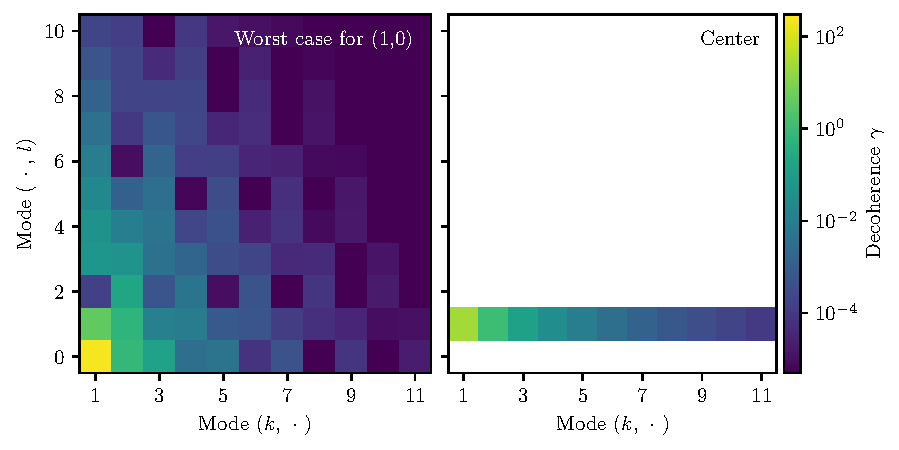
\includegraphics[width=\textwidth]{./../figures/vibrations/decoherence-analytical.pdf}
%   \caption{Maximum decoherence $\gamma$ at $4\si{K}$ for all modes if the cat-state is placed \textbf{left:} at the point with maximum gradient of the mode $(1,0)$ and \textbf{right:} in the center of the plate. It becomes evident, that only a few low modes play an actual role for the total dephasing.}
%   \label{fig:5:}
% \end{figure}


% \begin{figure}[!htbp]
%   \centering
%   \def\svgwidth{\textwidth}
%   \input{./../figures/plate-vibration.pdf_tex}
%   \caption{For a large shield, vibrations can be interpreted locally as if one mass was a distance $\Delta L$ further away from a shield and the other one $\Delta L$ closer and as if both masses would be rotated by an angle $\Delta \theta$.}
% \end{figure}

\section{Discussions on the shield} \label{sec:4:discussion}

- **Charged or uncharged**
Compare requirements in size and thickness as well as thermal vibrations, which are less a problem for smaller shields

- Small shield = local casimir effect. Compare with sec. 3.3

- How large are the effects of thermal vibration and how bad is everything
(Maybe in the next section, otherwise a little bit chaotic)

- Maybe a cross-structure or a different geometry of the shield could reduce vibrations and a larger shield might be okay. But local structures again

- Rectangular plate (frequencies only one order of magnitude ($\sqrt{\pi^4}$) better -> no real improvements)



% \begin{table}[!htbp]
%   \centering
%   \caption{large shield ($r_s \gg R$) and a small shield in the size of the particle size $r_s\sim R$. At $4\si{K}$.}
%   \begin{tabular}{l r c c c c c c}
%     \toprule
%     \multirow{3}{*}{Modes $(k,l)$} & \multicolumn{1}{c}{\multirow{3}{*}{Effect$^a$}} & \multicolumn{5}{c}{\textbf{large shield ($\mathbf{r_s \gg R}$)}} & \textbf{small shield} \\ %($\mathbf{r_s \sim R}$)
%     \cline{3-8}
%     & & \multicolumn{2}{c}{Worst position} && \multicolumn{2}{c}{Center$^b$} & \\
%     \cline{3-4} \cline{6-7}
%     & & $\Delta \theta/\Si{rad}$ & $\Delta L/\Si{m}$ && $\Delta \theta/\Si{rad}$ & $\Delta L/\Si{m}$ & $\Delta \theta/\Si{rad}$ \\
%     \midrule
%     $(1,0)$ & $97.66\,\%$ & $3 \times 10^{-7}$ & $9 \times 10^{-10}$ && - & $2 \times 10^{-9}$ & $2 \times 10^{-7}$ \\
%     $(1,1)$ &  $1.53\,\%$ & $8 \times 10^{-8}$ & $5 \times 10^{-10}$ && $2 \times 10^{-7}$ & - & $1 \times 10^{-7}$ \\
%     $(2,0)$ &  $0.32\,\%$ & $6 \times 10^{-8}$ & $1 \times 10^{-10}$ && - & $5 \times 10^{-10}$ & $1 \times 10^{-7}$ \\
%     $(2,1)$ &  $0.24\,\%$ & $8 \times 10^{-8}$ & $3 \times 10^{-11}$ && $1 \times 10^{-7}$ & - & $7 \times 10^{-8}$ \\
%     $(1,0)$ \& $(1,1)$ & $99.20\,\%$ \\
%     All above & $99.75\,\%$ \\
%     \bottomrule
%     \multicolumn{8}{l}{\footnotesize $^a$ Total effect on dephasing. Asymptotical scaling with $\mathcal{O}((k+l)^{-8})$}\\
%     \multicolumn{8}{l}{\footnotesize $^b$ Due to the symmetry, some modes don't contribute any variation in $\Delta\theta$ and $\Delta L$}
%   \end{tabular}
% \end{table}


\begin{table}[!htbp]
  \centering
  \caption{large shield ($r_s \gg R$) and a small shield in the size of the particle size $r_s\sim R$. At $4\si{K}$.}
  \begin{tabular}{l c c c c c c c}
    \toprule
    \multirow{3}{*}{Modes $(k,l)$} & \multicolumn{5}{c}{\textbf{large shield ($\mathbf{r_s \gg R}$)}} & & \textbf{small shield} \\ %($\mathbf{r_s \sim R}$)
    \cline{2-6} \cline{8-8}
    & \multicolumn{2}{c}{Maximum gradient} && \multicolumn{2}{c}{Center$^a$} && \\ % \multirow{2}{*}{$\Delta \theta/\Si{rad}$} \\
    \cline{2-3} \cline{5-6}
    & $\Delta \theta/\Si{rad}$ & $\Delta L/\Si{m}$ && $\Delta \theta/\Si{rad}$ & $\Delta L/\Si{m}$ && $\Delta \theta/\Si{rad}$ \\
    \midrule
    $(1,0)$ & $3.0 \times 10^{-7}$ & $9.3 \times 10^{-10}$ && - & $1.9 \times 10^{-9}$ && $1.9 \times 10^{-7}$ \\
    $(1,1)$ & $7.8 \times 10^{-8}$ & $4.8 \times 10^{-10}$ && $2.1 \times 10^{-7}$ & - && $1.3 \times 10^{-7}$ \\
    $(2,0)$ & $6.6 \times 10^{-8}$ & $1.7 \times 10^{-10}$ && - & $4.7 \times 10^{-10}$ && $1.0 \times 10^{-7}$ \\
    $(2,1)$ & $8.8 \times 10^{-8}$ & $3.5 \times 10^{-11}$ && $1.2 \times 10^{-7}$ & - && $7.5 \times 10^{-8}$ \\
    \hline
    $(1,0)$ \& $(1,1)$ & $3.8 \times 10^{-7}$ & $1.4 \times 10^{-9}$ && $2.1 \times 10^{-7}$ & $1.9 \times 10^{-9}$ && $3.2 \times 10^{-7}$\\
    \textbf{All above} & $\mathbf{5.3 \times 10^{-7}}$ & $\mathbf{1.6 \times 10^{-9}}$ && $\mathbf{3.3 \times 10^{-7}}$ & $\mathbf{2.4 \times 10^{-9}}$ && $\mathbf{4.9 \times 10^{-7}}$\\
    \bottomrule
    \multicolumn{8}{l}{\footnotesize $^a$ Due to the symmetry, some modes don't contribute any variation in $\Delta\theta$ and $\Delta L$}
  \end{tabular}
\end{table}